	\begin{frame}
		\frametitle{Focus: Theoretical Modelling}
		\vspace{12pt}
		\li{Lack of knowledge of the parton structure of the proton is the dominant source of uncertainty in the \wprime\, \& \zprime\, searches.}
		
		\li{Mass dependent corrections are applied to Monte Carlo in order to correct to current theory knowledge.}
		
		\cleft{.5}
			\li{Shift signal \& dominant background to best theory.}
			\lii{Signal: 	QCD {\scriptsize(NNLO)}.}
			\lii{CCDY BG : QCD {\scriptsize(NNLO)} \& EW {\scriptsize(NLO)}.}
			
			\li{Apply theoretical uncertainties for background predictions:}
			\lii{PDF \& $\alpha_{S}$ uncertainty for nominal PDF.}
			\lii{PDF choice uncertainty.}
		
		\vspace{-10pt}
		\begin{center}
		
		{\scriptsize{We calculate these uncertainties for the DY process and distribute them in widely used ATLAS tools.}}			\end{center}
		
		\cright{.5}
			\centering
			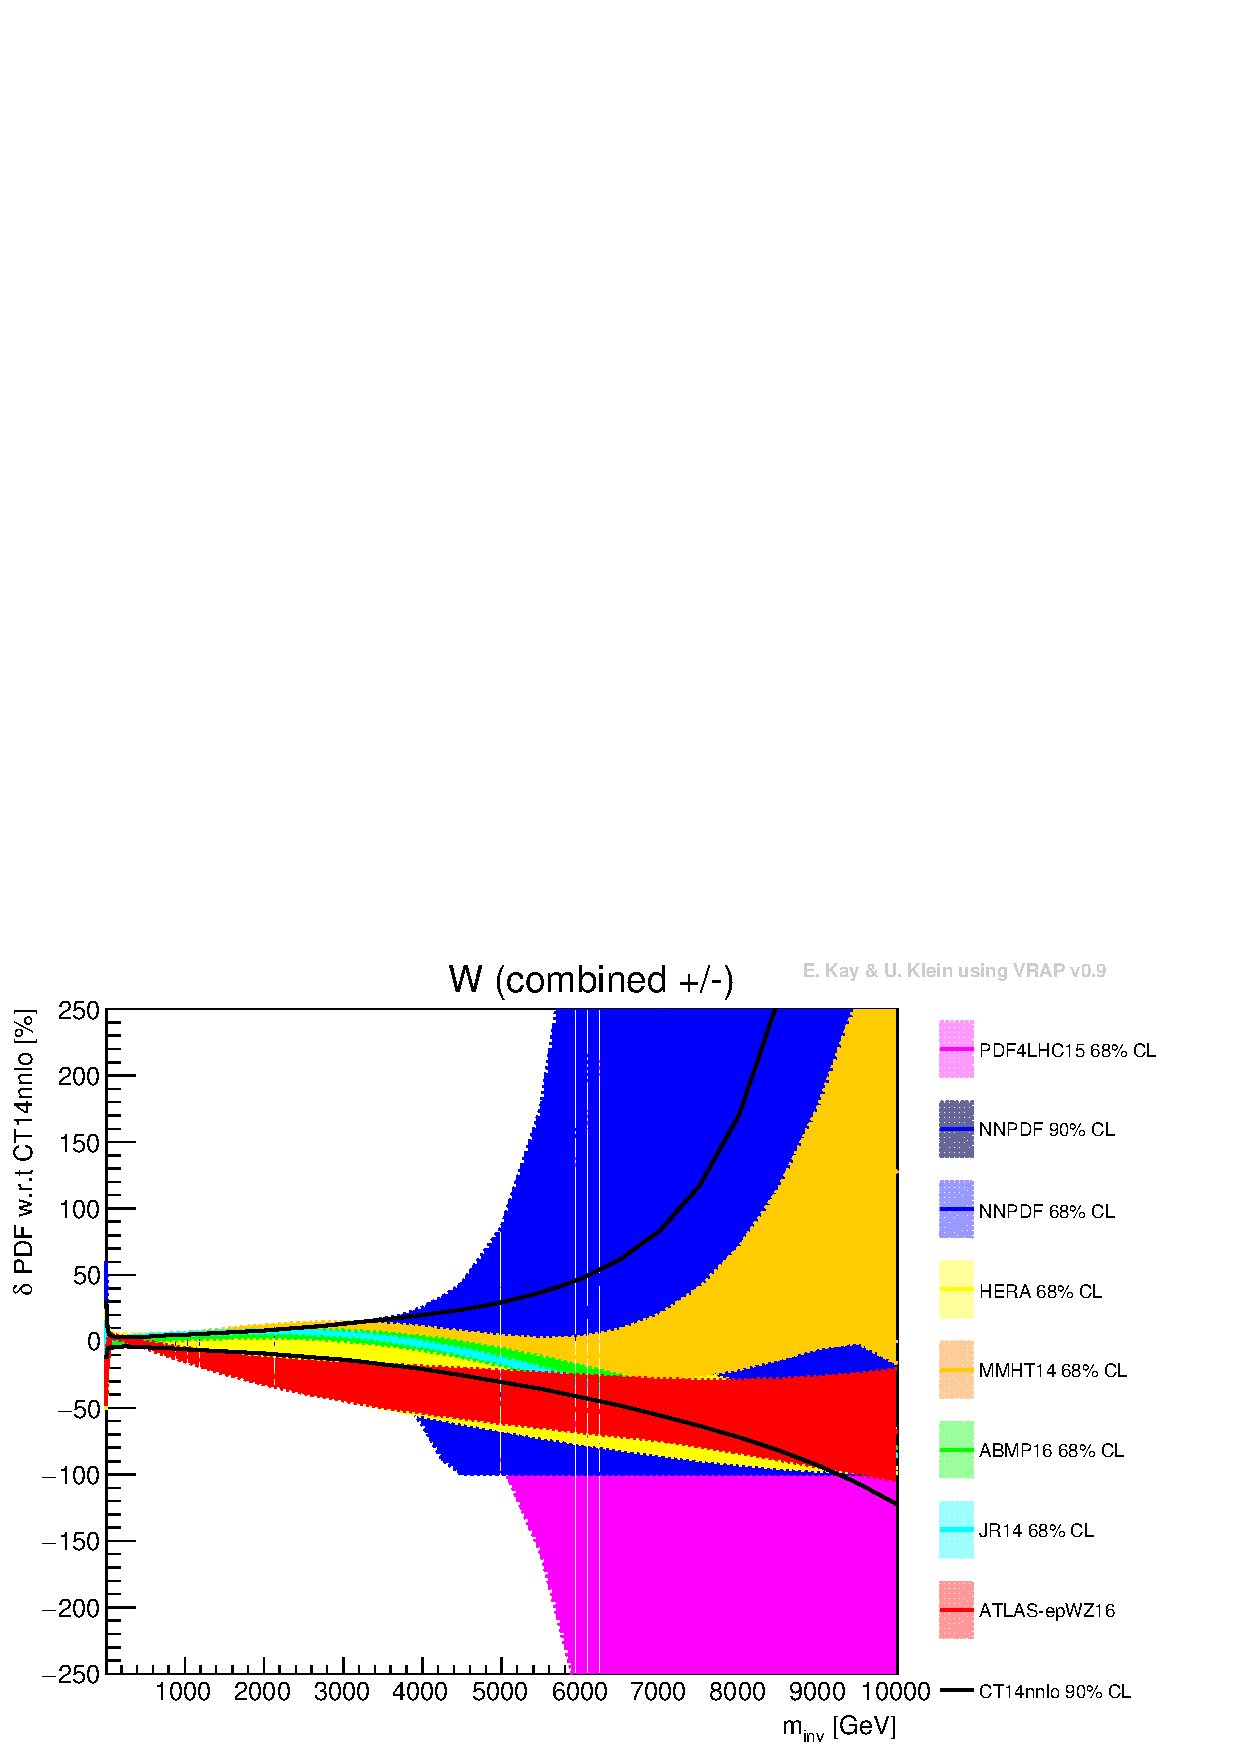
\includegraphics[height=\linewidth,angle=270]{plots/SUMMARY_ALLNEW/Wcomb.pdf}

		\cend
		
	
\end{frame}	